\onehalfspacing

User Story driven

\section{Lösungskonzepte}
\subsection{Openess-Kriterien}
\subsection{FAIR and CARE Principles}
\subsection{Wikimedia als Open Tech Stack}

\section{User Stories}

Strukturiert an idealtypischen Forschungsprozess

\subsection{User Story 1}

\subsection{User Story 2}

\subsection{User Story 3}

\subsection{User Story 4}

\subsection{User Story 5}

\section{Ergebnisse}

\begin{figure}[h]
\centering
\frame{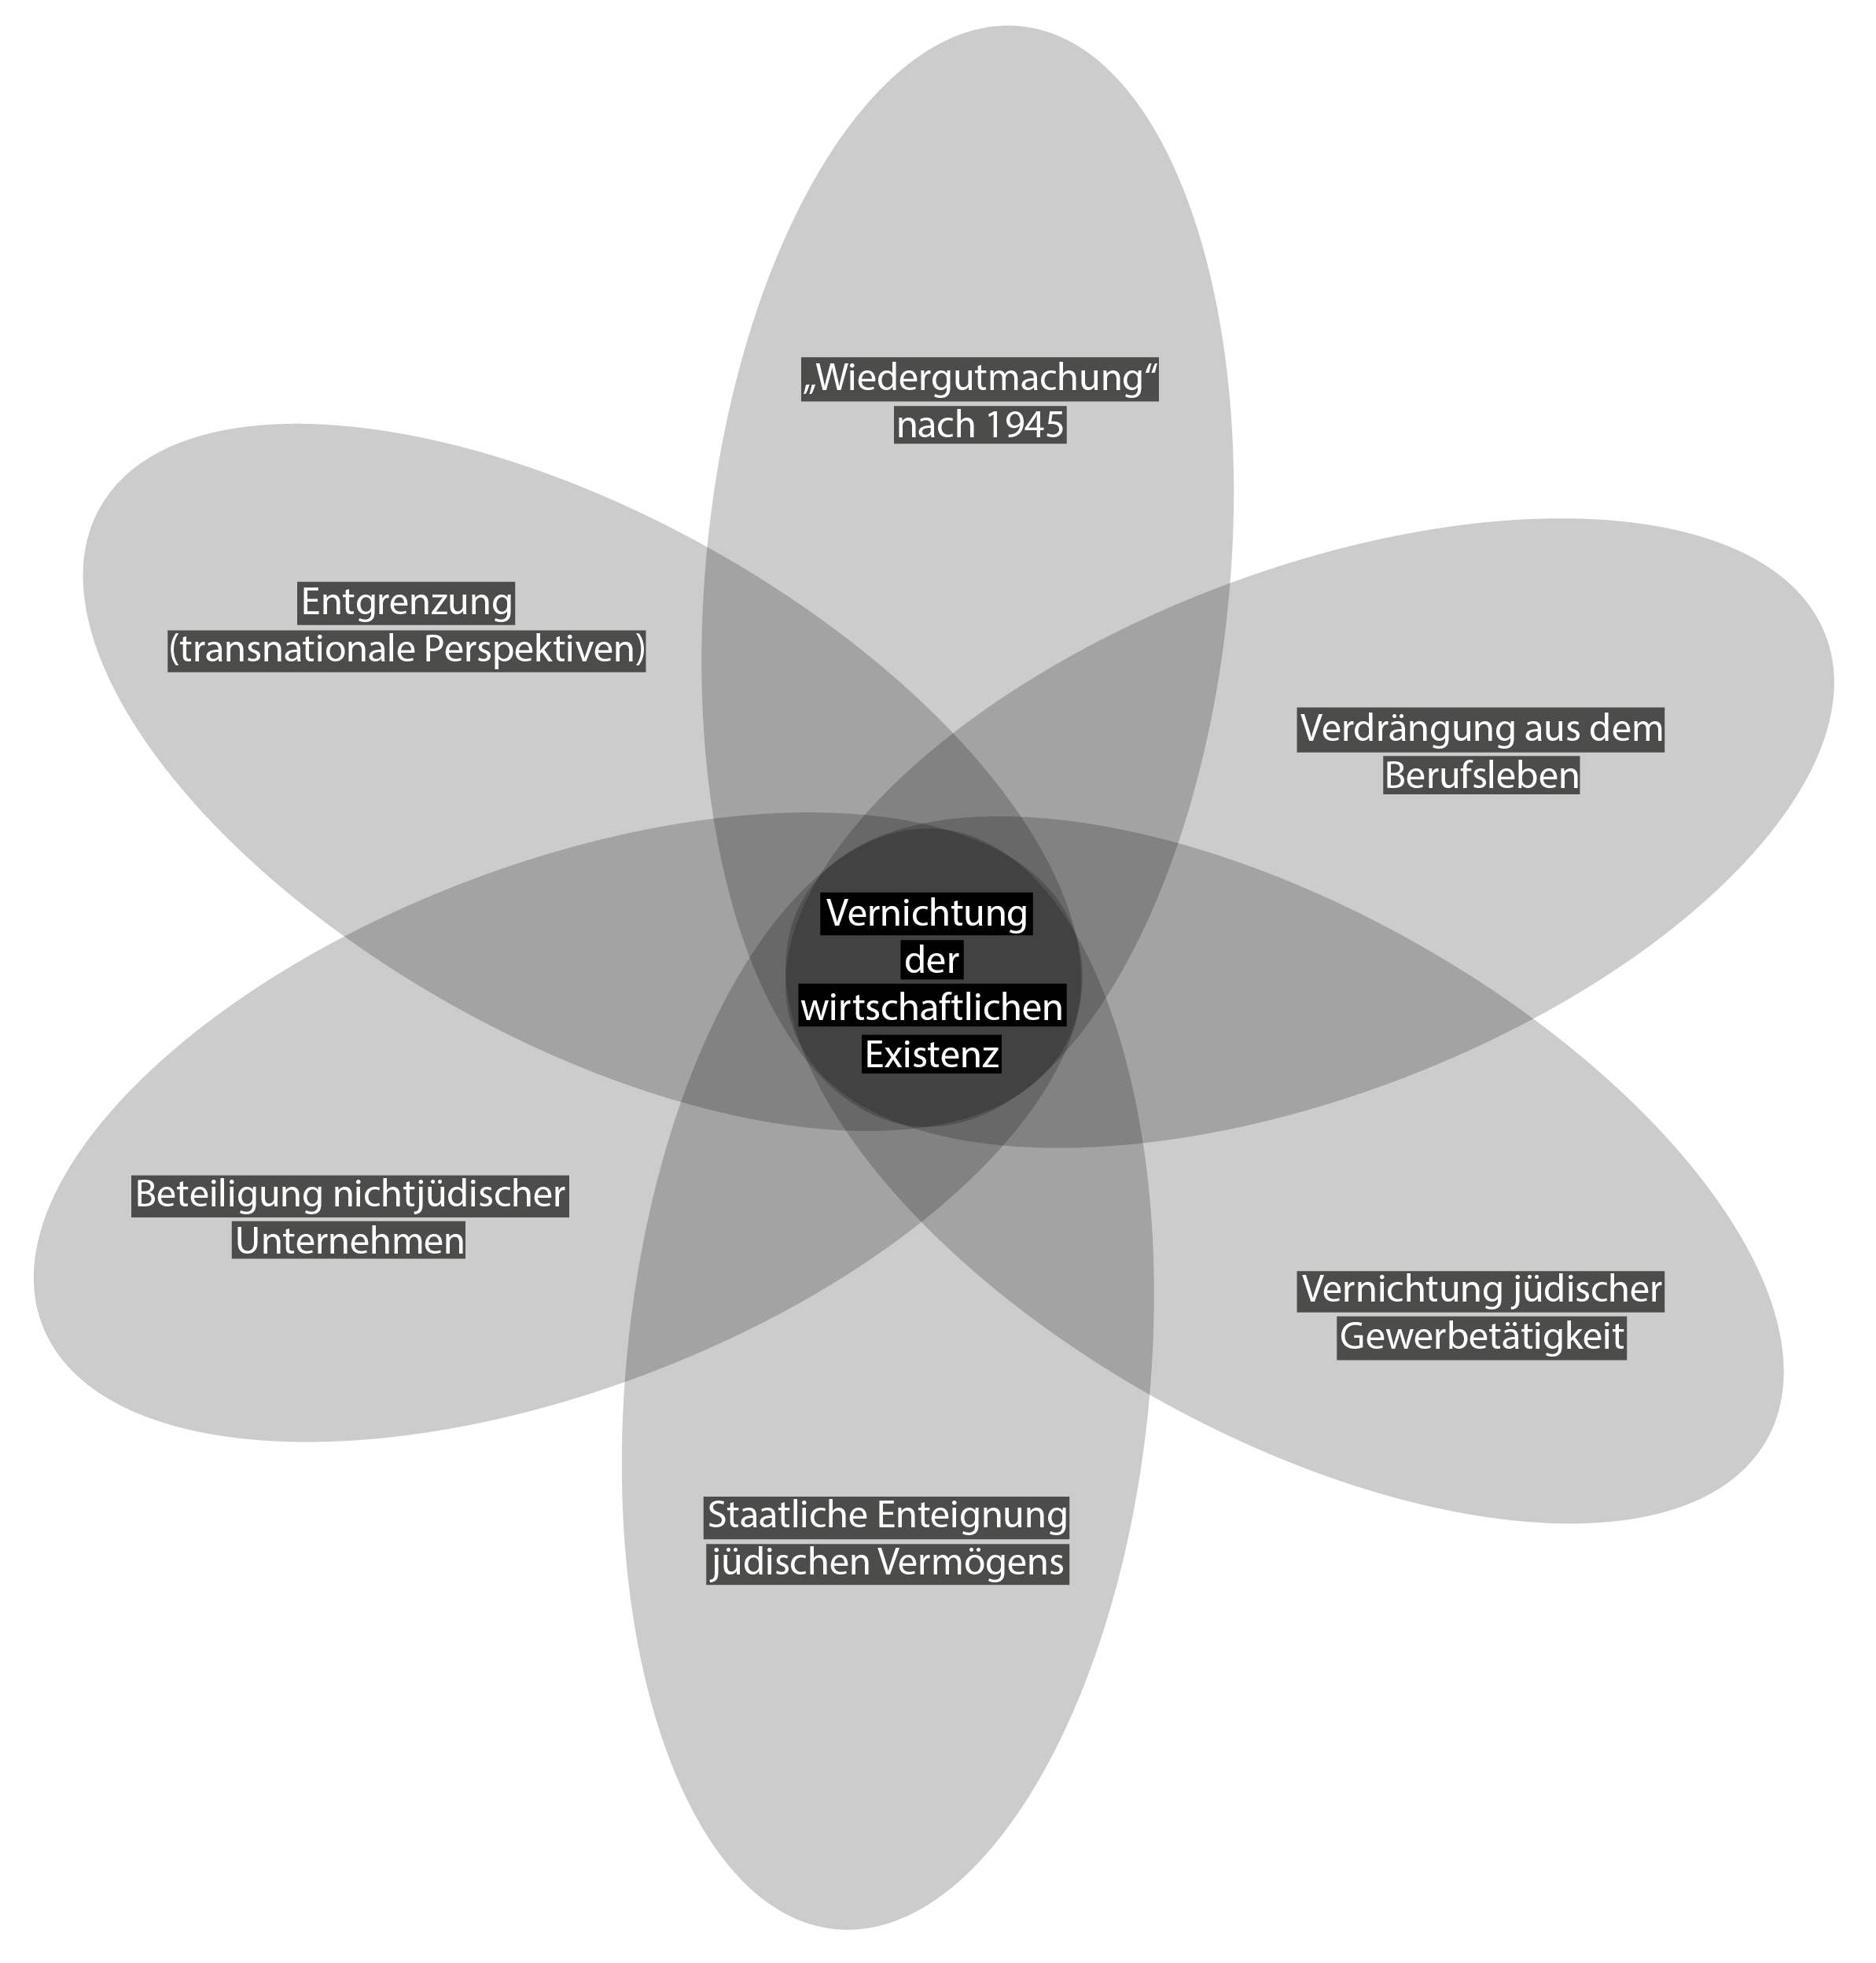
\includegraphics[scale=0.3]{Vernichtung_Gesamtprozess}}
\caption{Systematik des Forschungsfelds zur Vernichtung der wirtschaftlichen Existenz der deutschen Juden 1933-1945 nach Nietzel (2009), aufgeteilt nach fünf sich überlappenden Untersuchungsfeldern.\protect\footnote{Eigene Darstellung}}
\label{fig:x cubed graph}
\end{figure}

\begin{figure}[h]
\centering
\frame{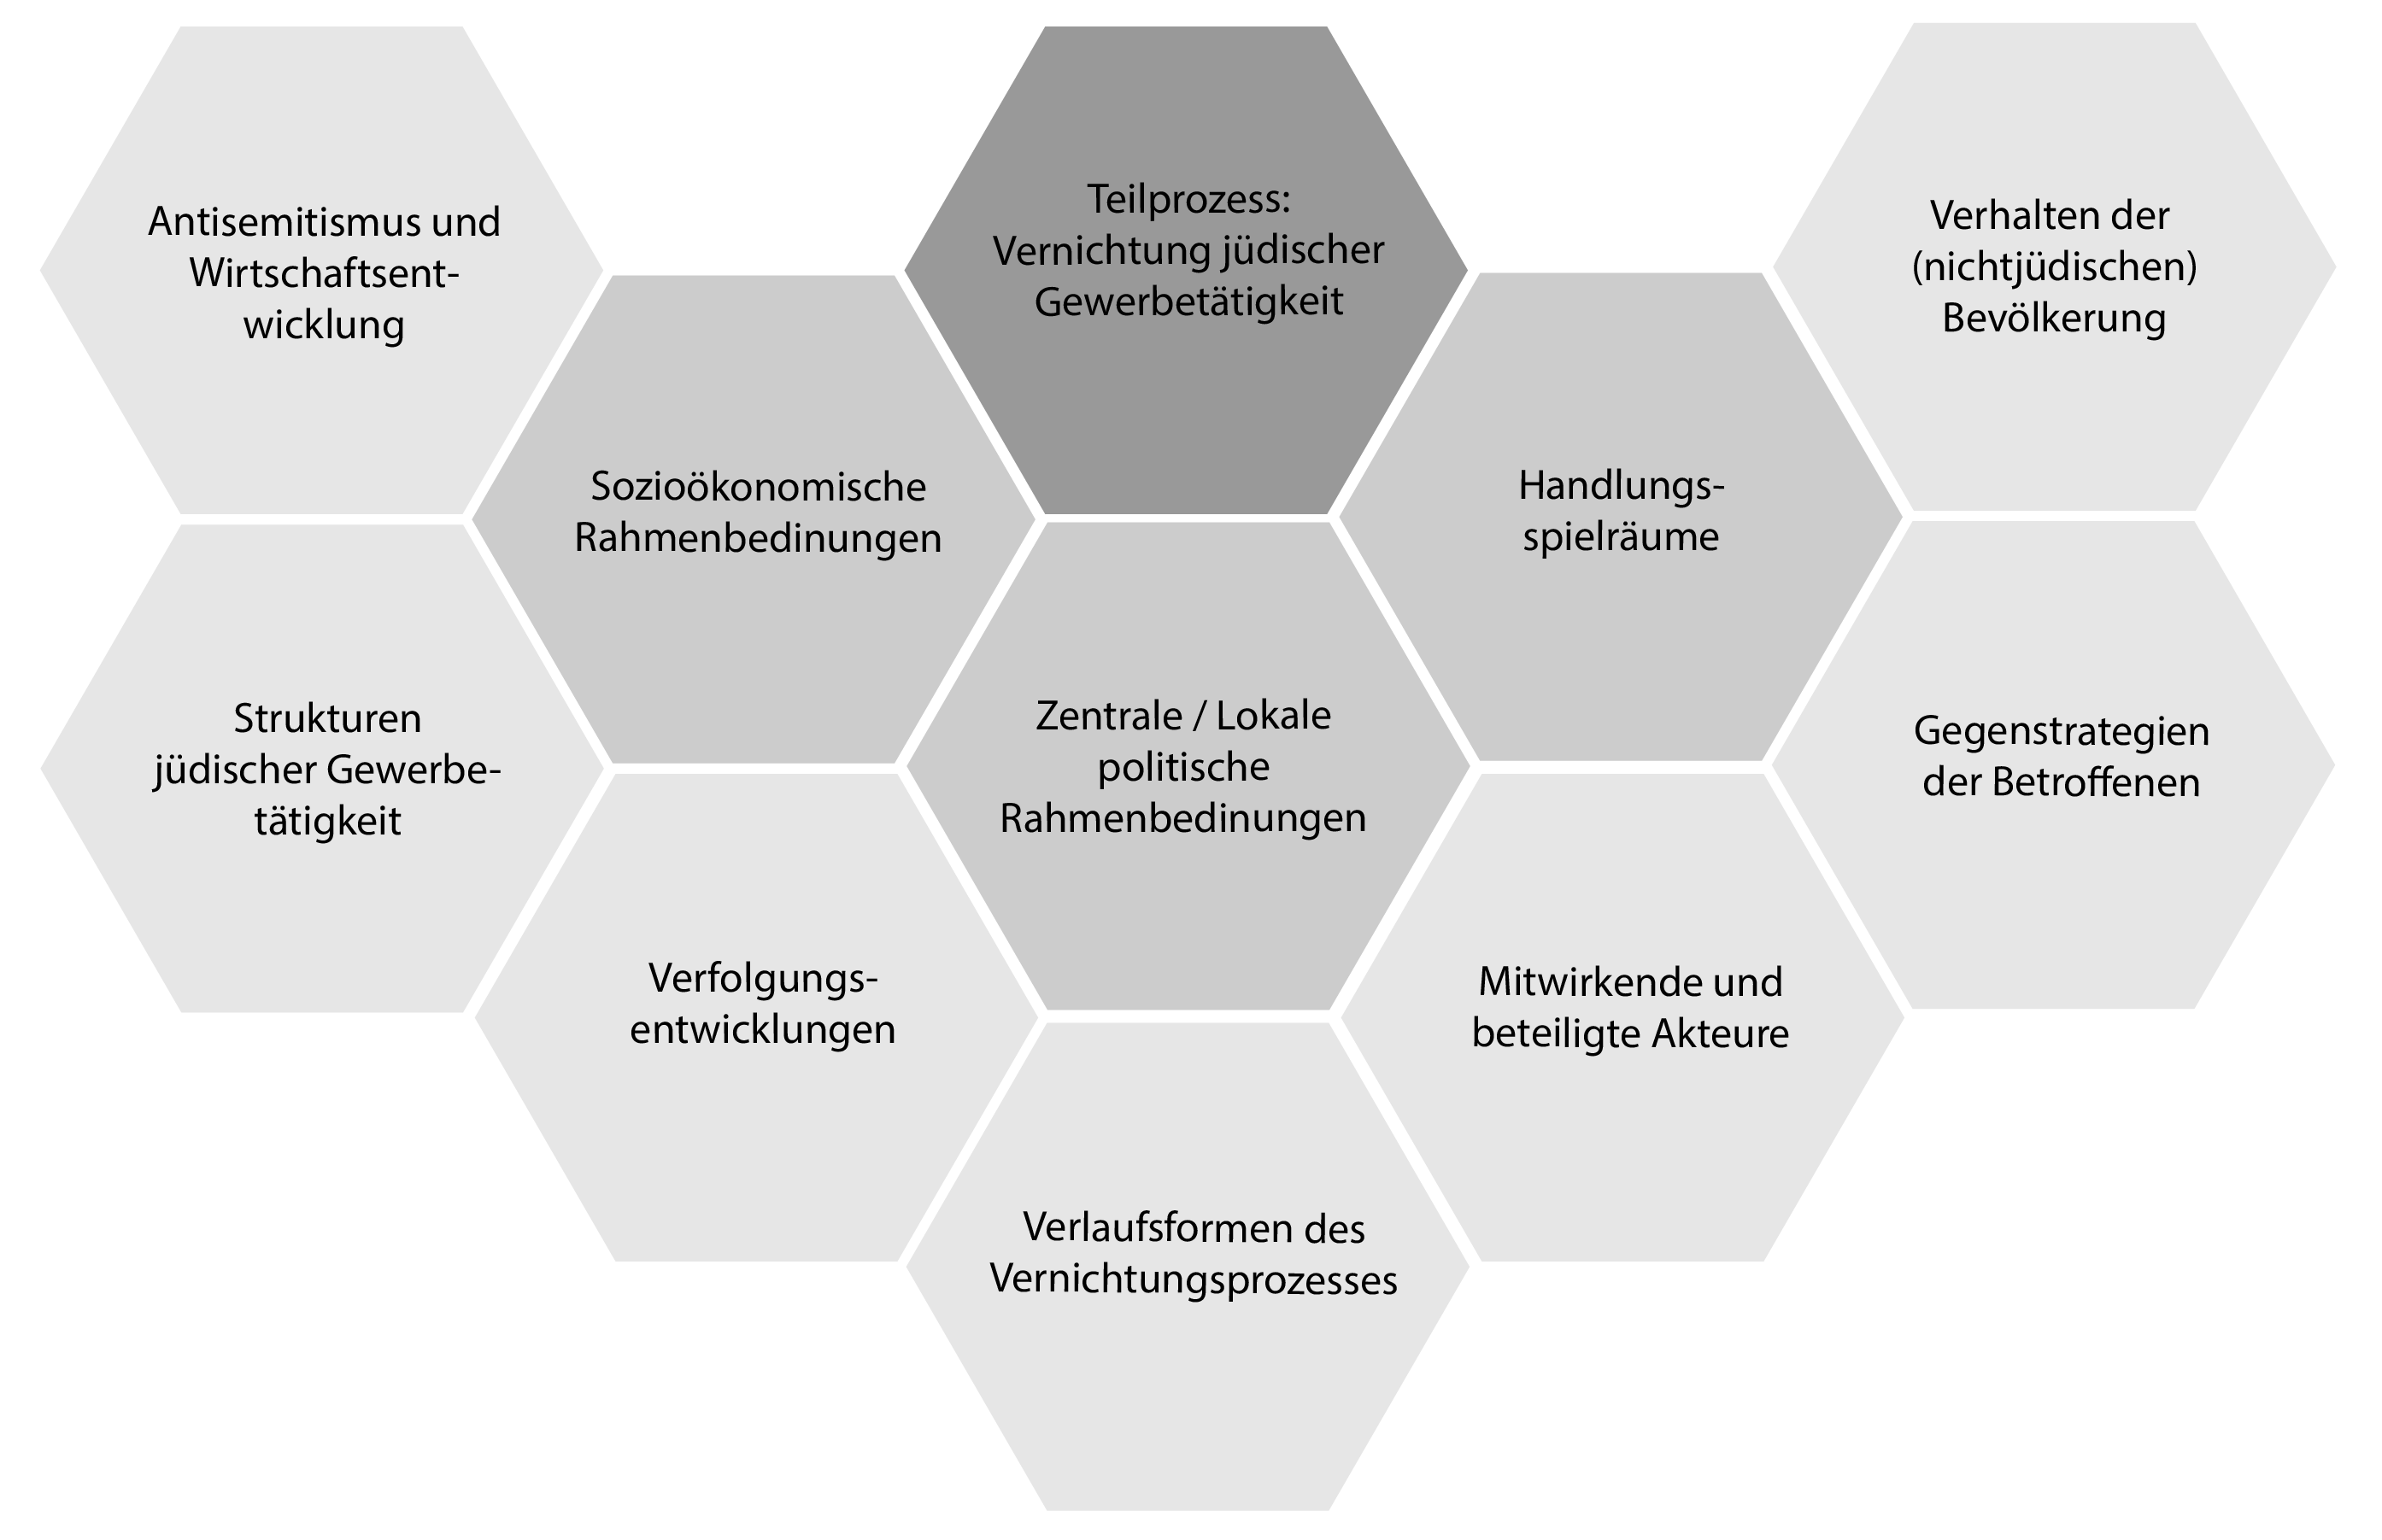
\includegraphics[scale=0.3]{Vernichtung_Teilprozess}}
\caption{Untersuchungsgebiete und Forschungsfragen des Forschungsfelds zur Vernichtung der jüdischen Gewerbetätigkeit 1933-45}
\label{fig:x cubed graph}
\end{figure}